\documentclass[a4paper, french]{report}

\usepackage[T1]{fontenc}
\usepackage[utf8]{inputenc} %caractères spéciaux
\usepackage[english, french]{babel} %français
\usepackage[left=2cm, right=2cm, top=2cm, bottom=2cm]{geometry}
\usepackage{graphicx}

\usepackage{amsmath}
\usepackage{amssymb}
\usepackage{mathrsfs} %maths

\usepackage{xspace} %symboles extensifs

\usepackage{listings}
\lstloadlanguages{[5.2]Mathematica}

\usepackage{eso-pic}
\newcommand\BackgroundPic{
\put(0,0){
\parbox[b][\paperheight]{\paperwidth}{%
\vfill
\centering
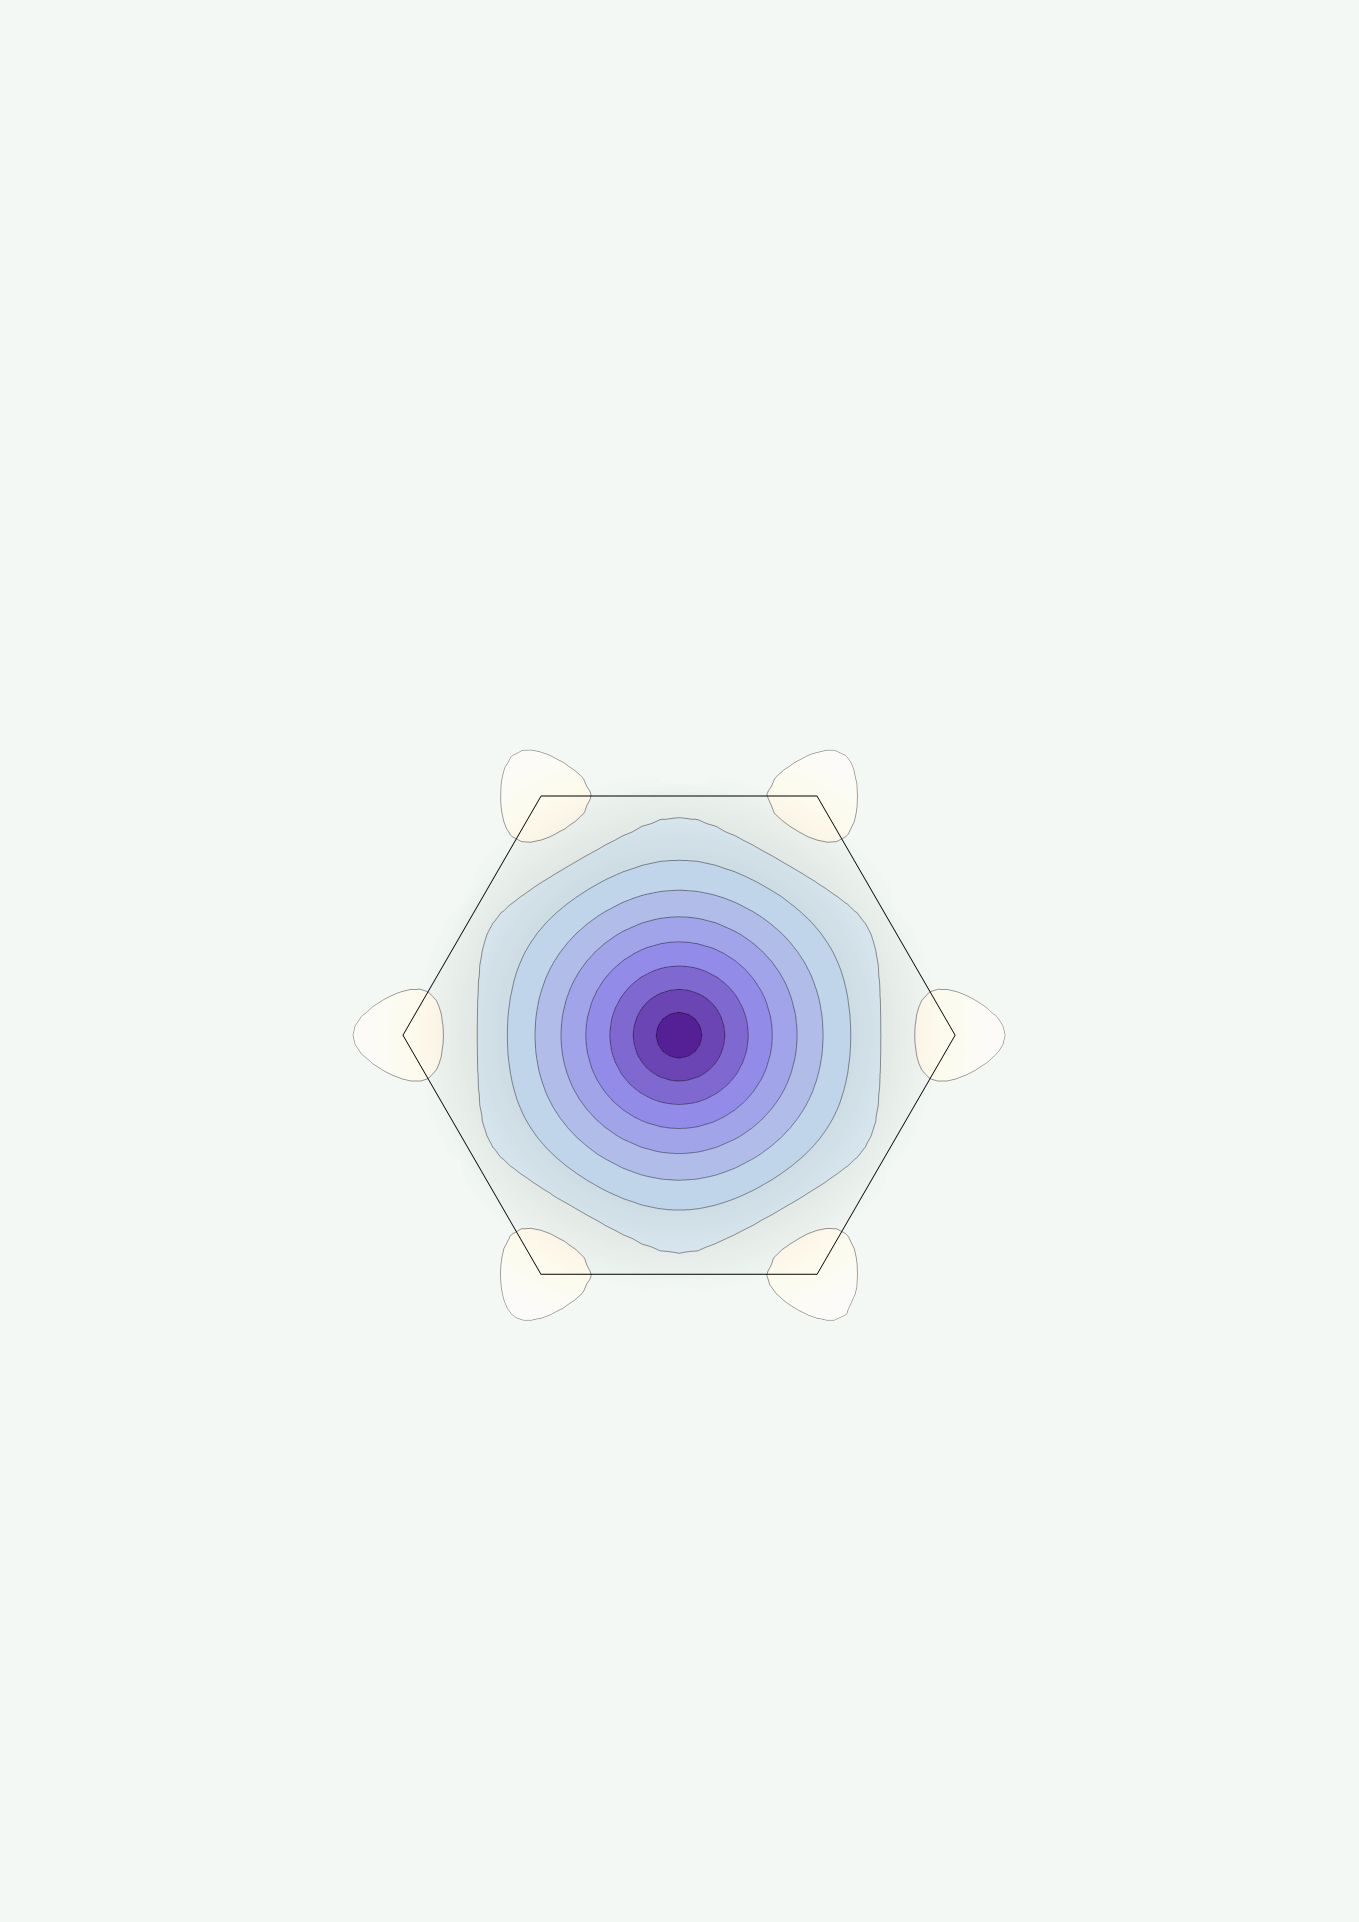
\includegraphics[width=\paperwidth,height=\paperheight,
keepaspectratio]{img_fond.png}%
\vfill
}}}

\newcommand{\ket}[1]{\ensuremath{|#1\rangle}\xspace}
\newcommand{\bra}[1]{\ensuremath{\langle #1|}\xspace}
\newcommand{\an}{\hat{a}}
\newcommand{\cre}{\hat{a}^\dagger}
\newcommand{\x}{\hat{x}}
\newcommand{\p}{\hat{p}}
\newcommand{\h}{\ensuremath{\hat{H}}\xspace}
\newcommand{\blbl}{création et annihilation }
\newcommand{\ban}{\hat{b}}
\newcommand{\bcre}{\hat{b}^\dagger}
\newcommand{\fond}{\ensuremath{| \Psi_0 \rangle}\xspace}
\newcommand{\pos}[1]{\ensuremath{\mathbf{r_{#1}}}\xspace}
\newcommand{\ond}{\ensuremath{\mathbf{k}\xspace}}
\newcommand{\A}{\ensuremath{{\mathbf{A}}}\xspace}
\newcommand{\B}{\ensuremath{{\mathbf{B}}}\xspace}
\newcommand{\M}[1]{\ensuremath{\mathbf{m}(#1)}\xspace}
\newcommand{\ank}{\an_{\ond}}
\newcommand{\crek}{\cre_{\ond}}
\newcommand{\bank}{\ban_{\ond}}
\newcommand{\bcrek}{\bcre_{\ond}}
\newcommand{\gam}{\gamma(\ond{})}
\newcommand{\alcre}{\hat{\alpha}^\dagger_{\ond}}
\newcommand{\alan}{\hat{\alpha}_{\ond}}
\newcommand{\betcre}{\hat{\beta}^\dagger_{\ond}}
\newcommand{\betan}{\hat{\beta}_{\ond}}
\newcommand{\om}{\ensuremath{\Omega}\xspace}
\newcommand{\bom}{\ensuremath{\bar{\Omega}}\xspace}
\newcommand{\1}{\ensuremath{\ket{\om_1\bom_1}}\xspace}
\newcommand{\2}{\ensuremath{\ket{\om_2\bom_2}}\xspace}
\newcommand{\spinu}{\ensuremath{\ket{\uparrow}}\xspace}
\newcommand{\spind}{\ensuremath{\ket{\downarrow}}\xspace}
\newcommand{\dens}{\ensuremath{\rho_0}\xspace}
\newcommand{\dred}{\ensuremath{\rho_{red}}\xspace}
\newcommand{\tr}{\text{tr}}
\newcommand{\struc}{structure en nid d'abeilles }
\newcommand{\tilm}{\ensuremath{\tilde{M}}\xspace}

\newcommand{\can}{\hat{c}}
\newcommand{\ccre}{\hat{c}^\dagger}
\newcommand{\ene}{\hat n}
\newcommand{\imp}[1]{\ensuremath{\mathbf{p_{#1}}}\xspace}
\newcommand{\Pos}[1]{\ensuremath{\mathbf{R_{#1}}}\xspace}

\begin{document}

\begin{titlepage}
\thispagestyle{empty}
\AddToShipoutPicture*{\BackgroundPic}


\begin{center}
\vspace{1.3cm}
{L3 de Physique
Fondamentale et Magistère 1}\\
\vspace{0.8cm}
{\Large{Stage du 23 mai au 4 juillet 2012}\\au Laboratoire de Physique des Solides, Orsay.}\\ 
\end{center}
\vspace{1.5cm}
\begin{center}
\rule{\textwidth}{1mm}
\Huge{\Huge \textbf{Entropie d'intrication dans un cristal antiferromagnétique bidimensionnel}} 
\rule[0.3cm]{\textwidth}{1mm}\\
\end{center}

\vspace{0.7cm}
\begin{tabular}{lll}
~\\
~\\
~\\
~\\
~\\
~\\
~\\
~\\
~\\
~\\
~\\
~\\
~\\
~\\
~\\
~\\
~\\
~\\
~\\
~\\
~\\
~\\
~\\
~\\
~\\
~\\
~\\
~\\
~
\end{tabular}
\begin{center}
\Large{\textbf{Stagiaire :} Nicolas Macé}\\
\Large{\textbf{Responsable de stage :} Anuradha Jagannathan}\\
\end{center}

\end{titlepage}
\pagebreak 

\selectlanguage{english}
\begin{abstract}
We study the gorund state of the antiferromagnetic Heisenberg hamiltonian, for a honeycomb lattice of spins 1/2. The entanglement entropy is given by $S(\Omega)=-\rho_{\Omega}\ln\rho_{\Omega}$, where $\rho_{\Omega}$ is the density matrix reduced to the subsystem \om. We find that $S$ is a linear function of the subsystem size, plus a logarithmic correction. We also compute the spin fluctuations in the ground state. It is found to be once again linearly dependant on the subsystem size, with a $L\ln L$ correction.

These results are compared with those recently found (april 2011 \cite{laflo}) for a square lattice.

\selectlanguage{french}
\begin{center}
\textbf{Résumé}
\end{center}
On s'intéresse à l'état fondamental de l'hamiltonien de Heisenberg antiferromagnétique pour des spins 1/2 sur un réseau bidimensionnel en nid d'abeilles. L'entropie d'intrication est donnée par $S(\Omega)=-\rho_{\Omega}\ln\rho_{\Omega}$,où $\rho_{\Omega}$ est l'opérateur densité réduit au sous système \om. On obtient que $S$ est une fonction linéaire de la taille du sous-système, plus une correction logarithmique. On calcule également les fluctuations des spins du sous-système dans l'état fondamental. On obtient là encore un terme fonction linéaire de la taille $L$, et une correction en $L \ln L$.

Les résultats sont comparés avec ceux obtenus récemment (avril 2011 \cite{laflo}) pour le réseau carré.
\end{abstract}

\selectlanguage{french}
\begin{center}
\Huge \textbf{Entropie d'intrication dans un cristal antiferromagnétique bidimensionnel}
\end{center}


\section*{\Huge{Introduction}}
Les systèmes étudiés en matière condensée (matériaux ferromagnétiques et antiferromagnétiques, supraconducteurs..) sont de vastes ensembles de corps en interaction. On sait depuis longtemps qu'à haute température, un modèle classique décrit bien ces systèmes, et permet d'en comprendre les propriétés. Plus récemment on s'est attaché à les décrire à basse température. Il est alors nécessaire de faire appel à un modèle quantique. La propriété d'intrication est une propriété nouvelle, purement quantique, qui apparaît dans ces modèles\cite{eisert, peschel}. L'étudier permettrait de mieux comprendre ces systèmes à basse température. On s'intéressera ici plus particulièrement à l'intrication dans un cristal antiferromagnétique bidimensionnel en nid d'abeilles à température nulle.

Dans une première partie, on verra comment décrire les cristaux ferromagnétiques et antiferromagnétiques dans le cadre du modèle de Heisenberg classique, puis quantique. Ensuite on se focalisera sur les cristaux antiferromagnétiques quantiques. On montrera comment, pour ces derniers, la transformation de Holstein-Primakoff permet de passer du modèle de Heisenberg à un modèle d'oscillateurs harmoniques couplés dont on souhaite calculer l'état fondamental.
Dans une deuxième partie on expliquera en détail ce qu'est l'entropie d'intrication.
Enfin, la troisième partie détaillera la méthode utilisée pour approcher numériquement l'entropie d'intrication à l'aide du logiciel Mathematica.

\tableofcontents

\chapter{Antiferromagnétiques quantiques}
\section{Modèle de Heisenberg}

Dans certains cristaux, et à basse température, l'agitation thermique n'est pas suffisante pour que les électrons soient itinérants. Ils demeurent au voisinage de leur atome. Cependant les atomes interagissent entre eux via le spin total de leur nuage électronique. C'est une interaction effective dûe au principe d'exclusion de Pauli et à l'interaction coulombienne. Pour deux atomes ayant des nuages électroniques de spins respectifs $\mathbf{S_1}$ et $\mathbf{S_2}$, on peut montrer que l'interaction effective prend la forme 
\begin{equation}
	\hat h=J\mathbf{S_1}\cdot \mathbf{S_2}
\end{equation}
où $J$ est une constante dépendant du recouvrement spatial des fonctions d'ondes des deux nuages électroniques.
Dans un cristal, si l'on suppose que les atomes interagissent deux à deux, et uniquement avec leurs plus proches voisins, l'interaction s'écrit
\begin{equation}
\label{eq:heis}
	\h=J\sum_{<i,j>}\mathbf{S_i\cdot S_j}
\end{equation}
C'est le modèle de Heisenberg isotrope. Le cristal décrit par un tel hamiltonien est généralement constitué d'un nombre macroscopique d'atomes, ce qui fait que l'on peut utiliser les outils de la physique statistique pour en trouver les propriétés. Voyons d'abord comment on peut attaquer classiquement le problème, avant de tenter de le faire quantiquement.

\subsection{Résolution classique à $T=0$}
\begin{figure}[htp]
\centering
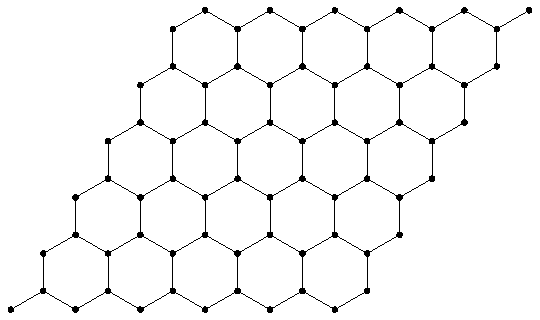
\includegraphics[scale=1.00]{vector_img/struc_nid_abeilles.pdf}
\caption{Structure en nid d'abeilles. Les positions des spins du réseau sont repérées par des cercles noirs, et les plus proches voisins sont reliés entre eux par des droites}
\label{1}
\end{figure}
Du point de vue classique, le spin n'est pas un opérateur mais un vecteur colinéaire au moment magnétique de l'atome. Le système que l'on étudie est un ensemble de spins localisés aux nœuds d'un réseau. (fig \ref{1})

Un microétat du système est donc la donnée des orientations de l'ensemble des vecteurs de spin. Plaçons nous dans l'ensemble canonique, ce qui revient à fixer la température $T$ du système. On pourrait, grâce aux outils de la physique statistique, calculer la fonction de partition du système, puis en déduire son énergie, son aimantation, etc. Nous nous contenterons ici de trouver son état fondamental, ie l'ensemble des microétats que peut occuper le système à température nulle.

La physique statistique nous dit que, si le nombre de spins est suffisamment grand, l'état physique dans lequel on va trouver le système est celui qui minimise l'énergie libre
\[
	F=\bar{E}-TS=\bar{E} \text{ car }T=0
\]
Il suffit donc de trouver l'ensemble des orientations des spins qui rendent $\bar{E}$ minimale.

Il y a deux cas de figure : $J<0$ ou $J>0$. Supposons tout d'abord que $J<0$.

Dans ce cas, le système est dans l'état fondamental si tous les spins sont parallèles. On dit que le cristal est \emph{ferromagnétique}. L'énergie du système dans l'état fondamental est
\begin{equation}
	H_{\text{spins parallèles}}=E_{cl}=JN_lS^2
\end{equation}
où $N_l$ est le nombre de liaisons et $E_{cl}$ l'énergie classique.


Supposons maintenant que $J>0$. Si on a la possibilité d'orienter chaque spin antiparallèlement avec ses voisins, alors on a caractérisé l'état fondamental. Son énergie est 
\begin{equation}
\label{eq:class}
	H_{\text{spins antiparallèles}}=E_{cl}=-JN_lS^2
\end{equation}
Il n'est cependant pas toujours possible d'orienter les spins de cette façon. (fig \ref{2})

\begin{figure}[htp]
\centering
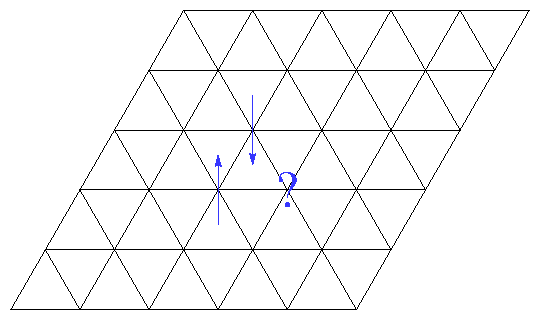
\includegraphics[scale=1.00]{vector_img/nobip.pdf}
\caption{Il n'est pas possible de positionner les spins antiparallèlement dans un réseau hexagonal.}
\label{2}
\end{figure}

Le cas qui nous intéresse est celui de la \struc antiferromagnétique. Pour ce réseau, il est possible d'orienter les spins antiparalèllement. (fig \ref{3})

\begin{figure}[htp]
\centering
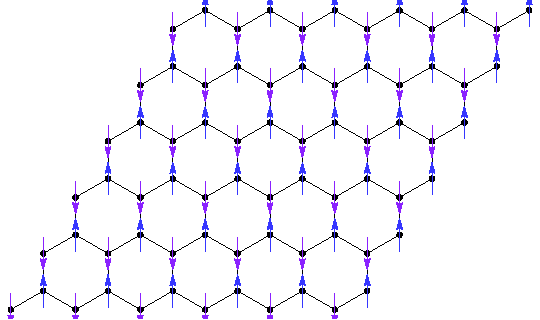
\includegraphics[scale=1.00]{vector_img/spins_struc_nid_abeilles.pdf}
\caption{Etat fondamental de la \struc antiferromagnétique. On voit apparaître deux sous-structures. Le réseau formé des spins vers le \og haut \fg{} (en bleu), et celle des spins vers le \og bas \fg{} (en violet). Ces deux structures sont des réseaux hexagonaux, qui seront respectivement appelés \emph{réseaux A et B} dans la suite.}
\label{3}
\end{figure}
On a donc trouvé l'ensemble des états fondamentaux classiques de notre problème ! Voyons maintenant ce qui se passe quantiquement.

\emph{Remarque :}
L'axe sur lequel les spins s'alignent (ou s'antialignent dans le cas antiferromagnétique) est arbitraire. Pourquoi les spins d'un cristal initialement à $T>0$ \og choisissent \fg{}-ils donc un axe plutôt qu'un autre lorsque l'on fait baisser la température du système jusqu'à atteindre $T=0$ ? En réalité, le cristal baigne toujours dans un champ magnétique résiduel $\mathbf{h}$ faible mais non nul. Les spins tendant à s'aligner dans le champ, c'est lui qui dicte leur orientation à $T=0$. Pour tenir compte de cela, introduisons dans le hamiltonien de Heisenberg un terme dû au champ magnétique extérieur dans lequel baigne le cristal :
\[
	\h=J\sum_{<i,j>}\mathbf{S_i\cdot S_j}+h\sum_{i}S_i^z
\]
(on a appelé $z$ l'axe du champ $\mathbf{h}$).
L'introduction de ce terme suffit à lever l'indétermination sur la direction et le sens des spins à température nulle dans le cas ferromagnétique. L'état fondamental est alors
\[
	\mathbf{S_i}=S_i^z\mathbf{e_z}=S\mathbf{e_z}
\]
Dans le cas antiferromagnétique en revanche, il subsiste une indétermination puisque les deux états \og spins du sous-réseau A dans le sens du champ et spin du sous-réseau B dans le sens opposé au champ \fg{} et \og spins du sous-réseau A dans le sens opposé au champ et spin du sous-réseau B dans le sens du champ \fg{} sont possibles. Pour lever complètement l'indétermination, on va plutôt introduire dans le hamiltonien une aimantation alternée :
\[
	\h_{antiferro}=J\sum_{<i,j>}\mathbf{S_i\cdot S_j}-h\sum_{i}(-1)^iS_i^z
\]

L'état fondamental est alors
\[
\left\{
	\begin{array}{r c l}
		\mathbf{S}=S_i^z\mathbf{e_z}=S\mathbf{e_z} \text{ si i désigne un point du réseau A}\\
		\mathbf{S}=S_i^z\mathbf{e_z}=-S\mathbf{e_z} \text{ si i désigne un point du réseau B}
	\end{array}
\right.
\]

En pratique on rajoute donc un terme de champ magnétique dans le hamiltonien antiferromagnétique. À la fin des calculs on passe à la limite thermodynamique, puis on fait $h\rightarrow 0$ pour l'éliminer des résultats. Comme dans la suite on ne donnera que les résultats, et pas les étapes de calcul, on ne fera pas apparaître le champ $\mathbf h$. Cependant il faut garder à l'esprit que c'est lui qui défini une direction et un sens privilégiés pour l'orientation des spins.

\subsection{Résolution quantique à $T=0$}
Les spins sont maintenant des opérateurs vectoriels, et plus des vecteurs. Le système est dans l'état fondamental si sa fonction d'onde est fonction propre du hamiltonien \ref{eq:heis} pour la plus basse énergie. On pourrait penser, par analogie avec le cas classique, que la fonction d'onde de l'état spins antiparallèles décrit l'état fondamental du système. Cependant ce n'est pas si simple. Comme on le verra par la suite, une telle fonction d'onde n'est pas fonction propre de $\h$ ! Il s'avère nécessaire de pousser les calculs pour trouver la fonctions d'onde de l'état fondamental. A l'heure actuelle pour une structure bidimensionnelle comme celle en nid d'abeilles, aucun calcul exact de la fonction d'onde de l'état fondamental n'existe. On peut cependant simplifier le problème en utilisant le développement en ondes de spins.

\section{Ondes de spins}
Notre objectif est de transformer le hamiltonien de Heisenberg
\[
	\h=J\sum_{<i,j>}\mathbf{S_i \cdot S_j}
\]
de façon à pouvoir trouver les propriétés de l'état fondamental.
L'idée du développement en ondes de spins est que :\\
1) L'énergie fondamentale quantique doit être proche de l'énergie fondamentale classique, que l'on connaît. Il faudrait donc trouver une transformation formelle de $\h$ qui fasse apparaît l'énergie classique \ref{eq:class}.\\
2) L'un des rares hamiltoniens quantiques que l'on sache diagonaliser est celui de l'oscillateur harmonique. Il serait donc utile de trouver une transformation formelle de $\h$ qui le fasse apparaître comme un hamiltonien d'oscillateurs harmoniques couplés.

La transformation de Holstein-Primakoff permet de réaliser cela.
\subsection{Transformation de Holstein-Primakoff}
Associons à chaque spin $\mathbf{S_i}$ du réseau des opérateurs création et annihilation notés $\cre_i$ et $\an_i$ pour les atomes du réseau A, $\bcre_i$ et $\ban_i$ pour les atomes du réseau B :

\begin{equation}
\label{eq:sz}
\left\{
	\begin{array}{r c l}
		S_i^z=S-\cre_i\an_i\\
		S_i^z=-S+\bcre_i\ban_i
	\end{array}
\right.
\end{equation}
La définition de ces opérateurs création et annihilation impose que :
\begin{equation}
\left\{
	\begin{array}{r c l}
		S_i^+=\sqrt{2S}\sqrt{1-\frac{\cre_i\an_i}{2S}}\an_i\\
		S_i^-=\sqrt{2S}\cre_i\sqrt{1-\frac{\cre_i\an_i}{2S}}\\
	\end{array}
\right.
\end{equation}
pour le réseau A,
\begin{equation}
\left\{
	\begin{array}{r c l}
		S_i^+=\sqrt{2S}\bcre_i\sqrt{1-\frac{\bcre_i\ban_i}{2S}}\\
		S_i^-=\sqrt{2S}\sqrt{1-\frac{\bcre_i\ban_i}{2S}}\ban_i\\
	\end{array}
\right.
\end{equation}
pour le réseau B. Comme 
\[
	\mathbf{S_i}\cdot\mathbf{S_j}=S_i^zS_j^z+\frac{1}{2}(S_i^+S_j^-+S_i^-S_j^+)
\]
on obtient pour le hamiltonien \ref{eq:heis} :
\begin{equation}
\label{eq:ondspin}
	\h=J\sum_{<i,j>}(S-\cre_i\an_i)(-S+\bcre_j\ban_j)+S\left(\sqrt{1-\frac{\cre_i\an_i}{2S}}\sqrt{1-\frac{\bcre_j\ban_j}{2S}}\an_i\ban_j+\cre_i\bcre_j\sqrt{1-\frac{\cre_i\an_i}{2S}}\sqrt{1-\frac{\bcre_j\ban_j}{2S}}\right)
\end{equation}

On a vu dans la partie précédente que l'état classique antiferromagnétique est l'état \og spins antialignés suivant $z$ \fg{}. On voit d'après \ref{eq:sz} qu'on retrouve cet état classique en faisant $\cre_i\an_i=\bcre_i\ban_i=0$. On s'attend à ce que l'état fondamental ne diffère pas tellement de l'état classique. On va donc supposer qu'à température nulle $<\cre_i\an_i>\ll S$, $<\bcre_i\ban_i>\ll S$. \footnote{Ici $<\hat A>$ désigne -et désignera toujours par la suite- la valeur moyenne de l'opérateur $\hat A$ dans l'état fondamental \fond. ie $<\hat A> = \bra{\Psi_0}\hat A \fond$.} Faisons un développement de l'expression \ref{eq:ondspin} dans cette limite :
\begin{equation}
\label{eq:ondspindl}
	\h_{\text{ondes de spins}}=E_{cl}+JS\sum_{<i,j>}\cre_i\an_i+\bcre_j\ban_j+\an_i\ban_j+\cre_i\bcre_j
\end{equation}
Le développement à l'ordre 1 en terme des opérateurs création et annihilation redonne l'énergie classique. Le développement à l'ordre 2 est appelé \emph{développement en ondes de spins}\footnote{Il s'agit en fait du premier ordre du développement en ondes de spins. Si on avait développé le Hamiltonien jusqu'à l'ordre 4 en terme des opérateurs création et annihilation, on aurait obtenu le deuxième ordre du développement en ondes de spins.}. Comme le hamiltonien \ref{eq:ondspindl} du développement en ondes de spins ne contient que des monômes d'ordre 0 ou 2 des opérateurs création et annihilation, il peut être vu comme le hamiltonien d'un ensemble d'oscillateurs harmoniques couplés. C'est le hamiltonien que nous avons utilisé pour les calculs menés au cours de ce stage. A partir de maintenant nous le noterons $\h$.

A ce stade du calcul, nous n'avons pas encore exploité le fait que le système étudié est un cristal. Il a donc une structure \emph{périodique}. La transformation en séries de Fourier permettra de faire apparaître les propriétés de symétrie qui en découlent.

\section{Réseau réciproque}

L'espace dans lequel vivent les transformées de Fourier des grandeurs fonctions des points du réseau est appelé réseau réciproque. Voyons comment on peut le construire.

\subsection{Construction du réseau}
Partant d'un point de l'espace bidimensionnel et de deux vecteurs notés $\mathbf{a}$ et $\mathbf{b}$ et appelés \emph{vecteurs primitifs}, on génère un réseau en réalisant toutes les translations de ce point d'un nombre entier de fois les vecteurs primitifs. Sur la figure \ref{fig:hexa}, on a représenté la construction du réseau hexagonal, dont les vecteurs primitifs sont séparés d'un angle de $\pi/3$.

Le réseau est la structure mathématique sous-jacente au cristal. On obtient le cristal en disposant sur le réseau les atomes qui le constituent. On dit qu'on décore le réseau avec un motif.

On peut ainsi obtenir la structure en nid d'abeilles en décorant un réseau hexagonal (figure \ref{fig:hexa}) avec un motif à deux atomes. La figure \ref{fig:all} montre le réseau hexagonal ainsi décoré. Les points du réseau A sont en bleu, ceux du réseau B, en violet. Les points du réseau hexagonal sous-jacent sont en noir. Le point du réseau repéré par l'entier $i$ est à la position \pos{i}.

\begin{figure}[htp]
\centering
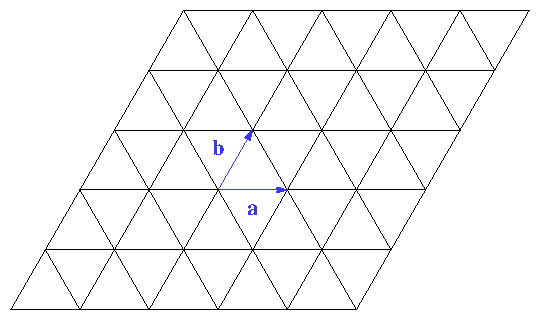
\includegraphics[scale=1.80]{vector_img/vect_prim_hexa.pdf}
\caption{Réseau hexagonal et ses vecteurs primitifs $\mathbf{a}$ et $\mathbf{b}$.}
\label{fig:hexa}
\end{figure}

\begin{figure}[htp]
\centering
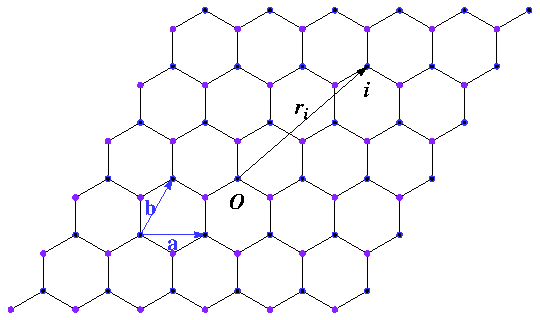
\includegraphics[scale=1.80]{vector_img/structure_nid_abeilles.pdf}
\caption{Réseau hexagonal décoré : structure en nid d'abeilles antiferromagnétique.}
\label{fig:all}
\end{figure}

\subsection{Réseau réciproque}
Utilisons le réseau le plus simple : la chaîne unidimensionnelle (fig \ref{fig:chain}) pour introduire la notion de réseau réciproque.
\begin{figure}[tp]
\centering
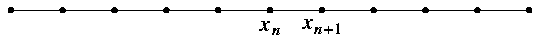
\includegraphics[scale=1.0]{vector_img/chaine.pdf}
\caption{Chaîne infinie d'atomes régulièrement espacés d'une distance $a$. Le n\up{ième} atome est à la position $x_n$.}
\label{fig:chain}
\end{figure} 
La distribution $F(x)=\sum_n\delta(x_n-x)$ contient toute l'information sur le réseau.
Prenons la transformée de Fourier de cette distribution :
\[
		TF(F)(k)=\sum_{n}e^{-ikx_n}=\sum_{n}e^{-ikna}
\]
Une somme infinie d'exponentielle est nulle, sauf si tous les termes de cette somme sont en phase, ie si $ka=2p\pi$, avec $p$ un entier relatif. L'ensemble des points $k$ ainsi obtenu est appelé \emph{réseau réciproque}.
La connaissance des réseaux direct et réciproque est équivalente : on passe de l'un à l'autre en prenant la TF ou la TF inverse de $F$.

Prenons une grandeur physique qui dépend de $x$, comme par exemple l'aimantation $\M{x_n}=<\mathbf{S_n}>$. Du fait de l'invariance par translation, une telle grandeur est périodique : $\M{x_n+a}=\M{x_n}$. On peut donc la décomposer en sérier de Fourier. Sa transformée de Fourier sera \emph{à valeurs dans l'espace réciproque}\footnote{$\sum_{k}$ désignera à partir de maintenant la somme sur tous les points de l'espace réciproque.}. Et on a
\begin{equation}
\label{eq:fourierinf}
	\M{x_n}=\sum_k\M{k}e^{ikx_n}
\end{equation}

\begin{figure}[htp]
\centering
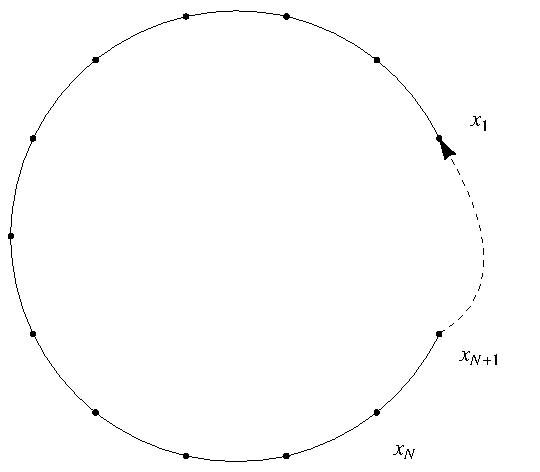
\includegraphics[scale=1]{vector_img/clp.pdf}
\caption{Chaîne de N atomes avec des conditions aux limites périodiques : on identifie le N+1\up{ième} atome avec le premier. Cela revient à refermer la chaîne sur elle-même.}
\label{fig:clp}
\end{figure}

En pratique on doit se limiter à un \emph{réseau de taille finie} avec des conditions aux limites périodiques (fig \ref{fig:clp}).
Les grandeurs physiques sont donc périodiques de période plus grande que dans le cas du réseau infini : $\M{x_n+(N+1)a}=\M{x_n}$.
La transformée de Fourier est toujours à valeur dans l'espace réciproque, qui est maintenant l'ensemble des $k=\frac{2p\pi}{Na}$. 
Comme \M{k} est $2\pi/(N+1)a$ périodique, on peut restreindre l'intervalle de variation de \M{k}, et de toutes les TF de grandeurs physiques, à un intervalle de longueur $2\pi/a$. On choisi traditionnellement l'intervalle centré sur l'origine. On l'appelle \emph{première zone de Brillouin}.

L'intérêt est que l'on peut remplacer la série de Fourier infinie \ref{eq:fourierinf} par une somme finie, qui porte uniquement sur les points $\ond$ de la première zone de Brillouin. Et on a
\begin{equation}
\left\{
	\begin{array}{r c l}
		\M{x_n}=\frac{1}{\sqrt{N}}\sum_{k}\M{k}e^{ikx_n}\\
		\M{k}=\frac{1}{\sqrt{N}}\sum_n\M{x_n}e^{-ikx_n}
	\end{array}
\right.
\end{equation}
où $N$ est le nombre de mailles.

\begin{figure}[htp]
\centering
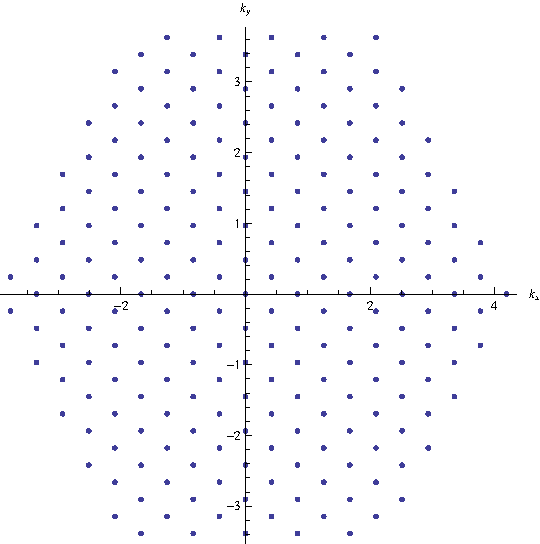
\includegraphics[scale=1]{vector_img/zone_brill.pdf}
\caption{Première zone de Brillouin pour la structure en nid d'abeilles. Les points correspondent aux valeurs de $k$ possibles pour un système fini de $N=100$ mailles. De manière générale, la première zone de Brillouin a toujours la même symétrie que le réseau. C'est ici c'est un hexagone, car la structure en nid d'abeilles repose sur un réseau hexagonal.}
\label{fig:zonebrill}
\end{figure}

Pour le cas qui nous intéresse, celui d'un réseau bidimensionnel, le raisonnement est strictement identique. Les TF sont maintenant des TF bidimensionnelles, et la première zone de Brillouin devient une surface de l'espace réciproque. Dans le cas de la structure en nid d'abeilles, c'est un hexagone (fig \ref{fig:zonebrill}).
\section{Hamiltonien du développement en ondes de spins dans l'espace réciproque}
Les opérateurs \blbl sont invariants par translation sur le réseau, on peut donc écrire leurs TF :
\begin{equation}
\left\{
	\begin{array}{r c l}
		\an_i=\frac{1}{\sqrt{N}}\sum_{\ond}\an_{\ond}e^{i\ond\cdot\pos{i}}\\
		\an_{\ond}=\frac{1}{\sqrt{N}}\sum_i\an_ie^{i\ond\cdot\pos{i}}
	\end{array}
\right.
\end{equation}
et de même pour $\bcre$ et $\ban$.


En remplaçant les opérateurs \blbl par leur développement en série de Fourier dans le hamiltonien \h, on obtient le hamiltonien dans l'espace réciproque :
\begin{equation}
	\h=E_{cl}+JSz\sum_{\ond}\crek\ank+\bcrek\bank+\gam^*\ank\bank+\gam\crek\bcrek
\end{equation}
où $z$ est le nombre de plus proches voisins d'un atome du cristal ($z=3$ pour la structure en nid d'abeilles), et où $\gam=\frac{1}{z}\sum_{\boldsymbol{\delta}}e^{i\ond\cdot\boldsymbol{\delta}}$

On a transformé la somme sur le plus proches voisins $\sum_{<i,j>}$ en une somme sur les vecteurs du réseau réciproque de la première zone de Brillouin $\sum_{\ond}$, qui est plus facile à manipuler. N'oublions pas que notre objectif est de trouver l'état fondamental du système. Si nous pouvions supprimer les termes non diagonaux du hamiltonien, ie trouver des opérateurs \blbl $\alan, \alcre, \betan, \betcre$ tels que $\crek\ank+\bcrek\bank+\gam^*\ank\bank+\gam\crek\bcrek=E_{\ond}\alcre\alan+E'_{\ond}\betcre\betan$, alors on pourrait voir l'état fondamental \fond comme l'état propre de valeur propre nulle de $\alcre\alan$ et de $\betcre\betan$.

\section{Transformation de Bogoliubov}
La transformation de Bogoliubov permet de supprimer les termes couplés de \h. Voyons comment elle opère.

Posons $\h_{\ond}=\crek\ank+\bcrek\bank+\gam^*\ank\bank+\gam\crek\bcrek$. On peut écrire $\h_{\ond}$ sous la forme
\begin{equation}
	\h_{\ond}=
	\begin{pmatrix}
	\cre & \ban\\
	\end{pmatrix}
	\underbrace{
	\begin{bmatrix}
	1 & \gam^*\\
	\gam & 1\\
	\end{bmatrix}
	}_{=M}
	\begin{pmatrix}
	\an\\
	\bcre\\
	\end{pmatrix}
\end{equation}
Notre but est de trouver une \emph{transformation canonique}\footnote{Une transformation canonique associe à des opérateurs création et annihilation (en l'occurrence $\ank$, $\crek$ et $\bank$, $\bcrek$) de nouveaux opérateurs (en l'occurrence $\alan$, $\alcre$ et $\betan$, $\betcre$) qui sont \emph{eux aussi} des opérateurs création et annihilation.} qui supprime les termes non diagonaux de $\h_{\ond}$. 
On peut montrer qu'on obtient la bonne transformation en diagonalisant $\tilde M=GM$ avec $G$ la matrice du commutateur :
\[
	G=
	\begin{bmatrix}
	[\an,\cre] & [\an,\ban]\\
	[\cre,\bcre] & [\bcre,\ban]\\
	\end{bmatrix}
	=
	\begin{bmatrix}
	1 & 0\\
	0 & -1\\
	\end{bmatrix}
\]
 
On obtient après calculs \footnote{Les calculs sont détaillés en Annexe A.}
\begin{equation}
\label{eq:ondspindecoupl}
	\h=E_{cl}-\frac{JSzN}{2}+JSz\sum_{\ond}E_{\ond}+JSz\sum_{\ond}E_{\ond}(\alcre\alan+\betcre\betan)
\end{equation}
où $E_{\ond}=\sqrt{1-|\gam|^2}$.


\begin{figure}[htp]
\centering
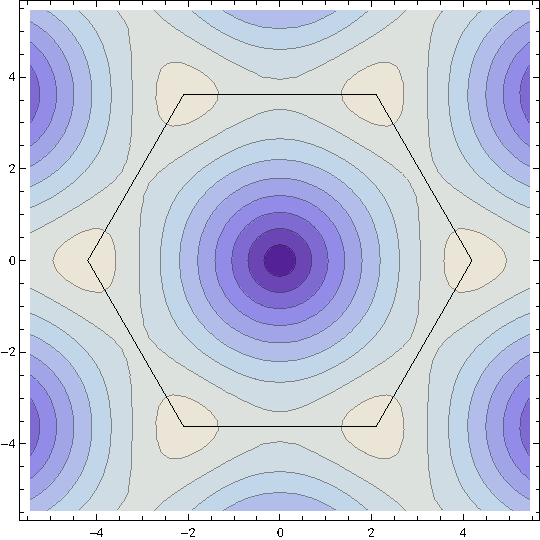
\includegraphics[scale=1.00]{vector_img/contour_energie_zone_brill.pdf}
\caption{Représentation de l'énergie $E_{\ond}$ dans l'espace réciproque. L'hexagone noir délimite la première zone de Brillouin. L'énergie est minimale au centre, maximale aux sommets de l'hexagone.}
\label{fig:energie}
\end{figure}

L'expression \ref{eq:ondspindecoupl} de \h permet de caractériser très facilement l'état fondamental. C'est l'état de plus basse énergie, donc tel que $\alcre\alan\fond=\betcre\betan\fond=0$. On en déduit l'énergie de l'état fondamental dans l'approximation des ondes de spins :
\begin{equation}
	E_{T=0}=\bra{\Psi_0}\h\fond=E_{cl}-\frac{JSzN}{2}+JSz\sum_{\ond}E_{\ond}
\end{equation}
Dans la limite où $E_{\ond}$ varie lentement avec $\ond$, on peut transformer la somme en intégrale.
\[
	\sum_{\ond}E_{\ond}=A\int \text{d\textbf{k}}\sqrt{1-|\gam|^2}
\]
où $A$ est l'aire du cristal. Une application numérique donne\\
\begin{tabular}{|c|c|}
\hline
	\textbf{Type de structure} & $\mathbf{E_{T=0}/N_l}$\\
\hline
	cristal classique antiferromagnétique & -0,25\\
\hline
	réseau carré antiferromagnétique  & -0,33\\
\hline
	structure en nid d'abeilles antiferromagnétique & -0,53\\
\hline
\end{tabular} avec $S=1/2$, $J=1$.
%Parler de l'état "spins liés 2 par 2 dans l'état singulet" quand z->0, de l'état classique quand z->infini

Pour la structure en nid d'abeilles (ainsi d'ailleurs que pour le réseau carré), l'énergie du développement en ondes de spins est inférieure à l'énergie classique ! L'état fondamental \fond n'est donc pas l'état classique \og spins antiparallèles \fg{}. Nous allons maintenant chercher à caractériser plus en détail l'état fondamental du système pour le réseau en nid d'abeilles, en calculant l'entropie d'intrication.

\chapter{Entropie d'intrication}

\begin{figure}[htp]
\centering
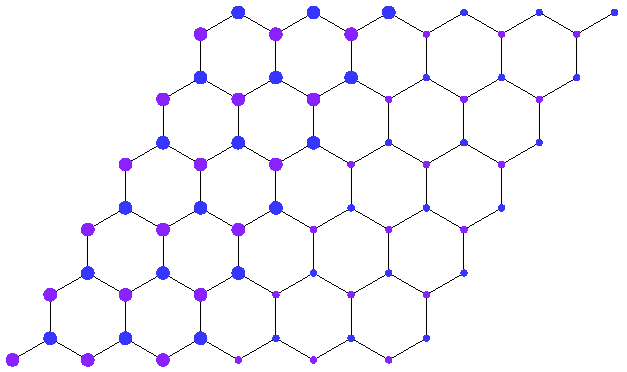
\includegraphics[scale=1.00]{vector_img/systeme_calculs.pdf}
\caption{Systèmes utilisés pour les calculs d'entropie d'intrication. Les points du système \om sont grossis par rapport à ceux du système \bom. On définit la \emph{taille du système total $\om \otimes\bom$} $L$ comme étant le nombre d'atomes sur l'un des axes du parralélogramme que constitue le système total. Sur la figure, $L=6$.}
\label{syst}
\end{figure}

Découpons par la pensée notre système, le cristal en deux sous-systèmes disjoints \om et \bom. L'espace de Hilbert $\mathcal{H}$ décrivant le système se factorise $\mathcal H=\mathcal H_{\om}\otimes\mathcal H_{\bom}$, où $\mathcal H_{\om}$ est l'espace décrivant le sous-système \om, $\mathcal H_{\bom}$ l'espace décrivant le sous-système \bom.

Imaginons que l'on ne puisse faire des mesures que sur le sous-système \om. En termes mathématiques, cela signifie que l'on ne peut connaître que la restriction à \om des observables qui caractérisent le système (aimantation, énergie, etc.). On a donc perdu une partie des informations sur le cristal. L'entropie d'intrication est la mesure de cette perte d'information.

On l'imagine sans mal, la perte d'information dépend pour un cristal donné de la taille relative des zones \om et \bom, mais aussi de leur forme. Par ailleurs la perte d'information dépend sans doute dans une certaine mesure de la structure du cristal (carré, nid d'abeilles, etc.). L'entropie d'intrication permettrait donc de mieux comprendre la structure des cristaux. Nous allons maintenant la calculer pour la structure en nid d'abeilles, et pour un type de sous-système particulier : celui constitué de la moitié du cristal. (voir figure \ref{syst})
Mais d'abord, voyons comment on peut trouver l'expression de l'entropie d'intrication dans un cas simplifié.

\section{Entropie d'intrication dans un cas simplifié}
Pour faire simple, imaginons que $\mathcal H_{\om}$ et $\mathcal H_{\bom}$ soient deux espaces de dimension 2, de bases respectives $(\ket{\om_1},\ket{\om_2})$ et $(\ket{\bom_1},\ket{\bom_2})$. Une base de $\mathcal H$ est donc $(\1,\ket{\om_1\bom_2},\ket{\om_2,\bom_1},\2)$. Supposons, là encore pour simplifier, que $\fond=\alpha\1+\beta\2$. L'opérateur densité \footnote{L'opérateur mathématique qui permet de décrire un système quantique qu'on ne connaît pas entièrement. Par ex. un électron dont on sait seulement que le spin a une chance sur 4 d'être \spinu et $3/4$ d'être \spind sera décrit par l'opérateur densité $\rho_{\text{électron}}=(1/4)\spinu\bra \uparrow+(3/4)\spind\bra \downarrow$. Ici, comme le système est de façon certaine dans l'état fondamental, l'opérateur densité est simplement $\dens=\fond\bra{\Psi_0}$. Voir \cite[pages~447-456]{basdevant} pour une introduction plus détaillée à la notion d'opérateur densité.} du système total \om$\otimes$\bom dans l'état fondamental est alors $\dens=\alpha^2\1\bra{\om_1\bom_1}+\alpha\beta(\1\bra{\om_2 \bom_2}+\2\bra{\om_1\bom_1})+\beta^2\2\bra{\om_2\bom_2}$.

Le système \om est décrit par l'\emph{opérateur densité réduit} \footnote{On peut montrer que l'opérateur densité décrivant le sous-système vivant dans un sous espace $\mathcal H_{\om}$ de l'espace de Hilbert total $\mathcal H_{\om}\otimes \mathcal H_{\bom}$ s'obtient en prenant la trace partielle de l'opérateur densité sur une base de $\mathcal H_{\bom}$. Ici, $\dred=\bra{\bom_1}\dens \ket{\bom_1}+\bra{\bom_2}\dens \ket{\bom_2}$.}
\[
	\dred=\alpha^2\1\bra{\om_1\bom_1}+\beta^2\2\bra{\om_2\bom_2}
\]

On voit que \dred est l'opérateur densité d'un mélange statistique : le sous-système \om a $\alpha^2$ chances d'être dans l'état $\ket{\om_1}$ et $\beta^2$ chances d'être dans l'état $\ket{\om_2}$. On a donc perdu de l'information par rapport à la situation où l'on pouvait connaître l'état du système total $\om \otimes \bom$. La perte est maximale si $\alpha=\beta=1/\sqrt{2}$, et minimale si $\alpha=0$ ou $\beta=0$.

La fonction 
\[
	S=-\alpha^2\ln(\alpha^2)-\beta^2\ln(\beta^2)
\]
caractérise bien la perte d'information : plus sa valeur est grande, plus cela signifie que l'on a perdu d'informations sur l'état du système. On l'appelle \emph{entropie d'intrication}.

On voit que l'on peut exprimer $S$ sous la forme 
\begin{equation}
	S=-\tr \dred \ln \dred
\end{equation}
où tr désigne la trace sur \bom.
Muni de cette expression commode -et valable dans le cas général- de l'entropie d'intrication, voyons comment on peut l'appliquer au système qui nous intéresse.

\section{Entropie d'intrication dans la structure en nid d'abeilles antiferromagnétique}
\label{sec:entnidabeilles}
Nous voulons reprendre les étapes de calculs du paragraphe précédent, qui nous ont mené à l'expression de $S$, avec cette fois le sous-système \om de la figure \ref{syst}.

Il s'agit tout d'abord de trouver l'état fondamental du système entier. On renvoie à l'annexe B pour la démontration de ce résultat. On trouve, en représentation position,
\begin{equation}
\label{eq:fond}
	\Psi_0(X)=C e^{-\frac{1}{2}X^TWX}
\end{equation}
où $C$ est une constante, $X$ le vecteur contenant les positions de tous les atomes du cristal :
\[
	X=
	\begin{pmatrix}
	\pos{1}\\
	\vdots\\
	\pos{2N}\\
	\end{pmatrix}
\]
et $W$ une matrice $2N\times 2N$ dépendant de la géométrie du réseau \footnote{Voir annexe C, section 2 pour plus de détails.}.
L'opérateur densité est donc donné -en représentation position- par
\begin{equation}
	\dens(X,X')=\Psi_0^*(X')\Psi_0(X)=C^2 e^{-\frac{1}{2}(X^TWX+X'^TTWX')}
\end{equation}

Il s'agit maintenant de déduire de \dens l'expression de l'opérateur densité réduit au sous-système \om. Là encore on renvoie à l'annexe B pour le détail des calculs. On trouve 
\begin{equation}
\label{eq:densred}
	\rho_{red}(x,x')=C^2\sqrt{Det(\frac{\pi}{W_{\bom\bom}})}\exp\left(-\frac{1}{2}(x^T(W_{\om\om})^{-1}x+x'^T(W_{\om\om})^{-1}x')+\frac{1}{4}(W_{\om\bom}(x+x'))^T(W^{-1}_{\bom\bom})^{-1}W_{\om\bom}(x+x')\right)
\end{equation}
Où $x,x'$ désignent les vecteurs contenant les positions de tous les atomes de \om, et où 
\[
	W=
	\begin{bmatrix}
	W_{\om\om} & W_{\om\bom}\\
	W_{\bom\om} & W_{\bom\bom}\\
\end{bmatrix}
\]

Enfin nous pouvons déduire de cela, en utilisant la formule \ref{eq:densred}, l'expression qui nous intéresse : celle de l'entropie d'intrication.
On trouve
\begin{equation}
\label{eq:ent}
	S=\sum_{q} \left(\nu_q+\frac{1}{2}\right)\ln \left(\nu_q+\frac{1}{2}\right)-\left(\nu_q-\frac{1}{2}\right)\ln \left(\nu_q-\frac{1}{2}\right)
\end{equation}
Où les $\nu_q$ sont les racines des valeurs propres de $1/4(W^{-1})_{\om\om}W_{\om\om}$. Nous avions dit que $W$, et par conséquent $W_{\om\om}$ et $(W^-1)_{\om\om}$, sont des matrices qui dépendent de la géométrie du réseau. Or c'est cela que l'on cherche à analyser ! Plus précisément on voudrait savoir, par exemple, comment l'entropie d'intrication évolue à mesure que l'on augmente la taille du cristal, et comparer cette évolution avec celle du réseau carré, que l'on connaît déjà. C'est en analysant les points communs et les différences d'allures entre les deux courbes d'évolution que l'on espère mieux comprendre comment se comportent de tels cristaux antiferromagnétiques à basse température.

Cependant, on ne voit pas très bien comment expliciter la dépendance de l'entropie en la taille du cristal à partir de l'équation \ref{eq:ent}. Nous allons donc calculer numériquement l'entropie d'intrication, pour des systèmes de plus en plus grands. On obtiendra ainsi la courbe d'évolution de l'entropie en fonction de la taille.

\chapter{Calculs numériques et résultats}
On a utilisé le logiciel Mathematica pour les calculs numériques. Le programme utilisé (et réalisé au cours du stage) est donné en annexe. Nous allons maintenant détailler le principe du programme, et discuter les résultats obtenus.

\section{Principe du programme}
\label{sec:pcppgrm}
Le système choisi pour les calculs est celui de la figure \ref{syst} : un parallélogramme de taille $L \times L$. Le sous-système \om est de taille $L/2 \times L$.

Notre objectif est de calculer, pour des valeurs de $L$ de plus en plus grandes, l'entropie d'intrication du sous-système \om, et une autre grandeur intéressante, la \emph{fonction des fluctuations} :
\begin{equation}
	F=\sum_{i,j \in \om} <S_i^zS_j^z>-<S_i^z><S_j^z>
\end{equation}
Quelle est la signification physique de $F$ ? Imaginons pour simplifier que l'on ait 2 spins $S_1$ et $S_2$.
		\begin{itemize}
			\item Si les spins sont proches voisins, ils sentiront une interaction effective antiferromagnétique $H=J\mathbf{S_1}\cdot\mathbf{S_2}$. À $T=0$ le système des deux spins est donc dans l'état singulet $\linebreak[4] \ket{\Psi_S}=(1/\sqrt{2})(\ket{\uparrow \downarrow}-\ket{\downarrow \uparrow})$ puisque c'est l'état qui minimise $H$. Donc $F_{\text{proches voisins}}=1$.
			\item À l'inverse si les spins sont très éloignés, ils n'interagissent pas et toutes les directions d'orientation des vecteurs de spins sont équiprobables. Cela est décrit par l'opérateur densité $\rho=\text{diag}(1/4,1/4,1/4,1/4)$. Et on a cette fois $F_{\text{spins éloignés}}=0$.
		\end{itemize}
$F$ décrit donc à quel point les spins de \om sont corrélés. 
$F$ peut aussi s'écrire \footnote{Voir démonstration en annexe C.}
\begin{equation}
\label{eq:fluctfg}
	F=\sum_{i,j} -\delta_{ij}/4+f(\pos{i}-\pos{j})^2-g(\pos{i}-\pos{j})^2
\end{equation}
où
\begin{equation}
\label{eq:fg}
\left\{
	\begin{array}{r c l}
		f(\pos{i}-\pos{j})=\frac{1}{N}\sum_{\ond{}} \frac{\exp{i\ond\cdot(\pos{i}-\pos{j})}}{\sqrt{1-|\gam|^2}}\\
		g(\pos{i}-\pos{j})=-\frac{1}{N}\sum_{\ond{}} \frac{\gam \exp{i\ond\cdot(\pos{i}-\pos{j})}}{\sqrt{1-|\gam|^2}}
	\end{array}
\right.
\end{equation}
Il est aisé d'évaluer numériquement $f$ et $g$ à l'aide de Mathematica. On en déduit la valeur numérique de $F$.

L'entropie d'intrication peut aussi s'exprimer à l'aide de $f$ et $g$. En effet ces deux fonctions sont reliées à la matrice $W$. Si on défini les matrices $X$ et $P$ par 
\begin{equation}
\label{eq:XP}
\left\{
	\begin{array}{r c l}
		X=
		\begin{bmatrix}
		F & G\\
		G & F\\
		\end{bmatrix}\\
		P=
		\begin{bmatrix}
		F & -G\\
		-G & F\\
		\end{bmatrix}
	\end{array}
\right.
\end{equation}
où $F_{ij}=f(\pos{i}-\pos{j})$ et $G_{ij}=g(\pos{i}-\pos{j})$,\\
alors $X=(1/2)W^{-1}_{\om\om}$ et $P=(1/2)W_{\om\om}$ \footnote{Voir démonstration en annexe C.} et donc les racines des valeurs propres de $XP$ sont exactement les $\nu_q$. On peut ainsi calculer numériquement l'entropie d'intrication $S$.
\section{Résultats}
\label{sec:res}
On a tracé $F$ et $S$ en fonction de la taille $L$ du cristal, en choisissant comme système et comme sous-système ceux de la figure \ref{syst}. Afin de pouvoir comparer nos résultats avec ceux déjà obtenus pour le réseau carré, nous avons utilisé les mêmes fonctions d'ajustement.

On approxime $F$ par la fonction $F(L)=a_FL \ln L +b_FL+c_F$, et l'entropie par la fonction $S(L)=a_S\ln L +b_SL+c_S$. Les valeurs des paramètres $a_L$, $b_L$, ... sont obtenues avec Mathematica. Elles sont portées sur les figures \ref{res1} et \ref{res2}. 

\begin{figure}[htp]
\centering
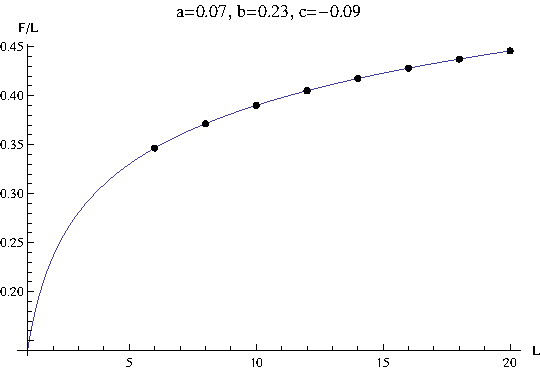
\includegraphics[scale=1.00]{vector_img/fluct.pdf}
\caption{Fonction des fluctuations divisée par la taille $L$ du système, en fonction de $L$.}
\label{res1}
\end{figure}

\begin{figure}[htp]
\centering
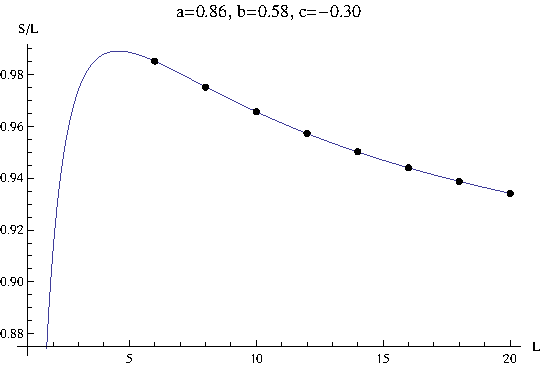
\includegraphics[scale=1.00]{vector_img/ent.pdf}
\caption{Entropie divisée par la taille $L$ du système, en fonction de $L$.}
\label{res2}
\end{figure}

Il faudrait, pour conforter les résultats obtenus pour les valeurs des paramètres d'ajustement, continuer les calculs numériques pour des valeurs de taille $L$ plus grandes. Il serait aussi bon de comparer ces résultats obtenus par la méthode du développement en ondes de spins -qui n'est qu'une approximation du modèle de Heisenberg- avec ceux obtenus par une autre méthode. Dans cette optique, des calculs numériques utilisant la méthode de Monte-Carlo quantique sont actuellement en train d'être réalisés par Nicolas Laflorencie, l'un des auteurs de \cite{laflo}.

Cependant on peut d'ores et déjà analyser les résultats que nous avons obtenus au cours de ce stage. On trouve $a_S \simeq 0.9$, valeur identique à celle trouvée dans \cite{laflo} pour le réseau carré antiferromagnétique. Cela laisse penser que la valeur du coefficient du terme logarithmique de l'entropie d'intrication est \emph{universelle} : indépendante de la géométrie du cristal bidimensionnel considéré\footnote{On peut démontrer que pour des cristaux unidimensionnels, ce coefficient est effectivement universel. Cela corrobore également notre hypothèse.}.
A l'inverse, les valeurs des coefficients de $F$ sont différentes de celles trouvées en \cite{laflo} pour le réseau carré antiferromagnétique. Cela signifie que $F$ est probablement une quantité non universelle.

\section*{\Huge Conclusion}
Nous sommes parti du modèle de Heisenberg antiferromagnétique. Nous en avons dérivé le hamiltonien du développement en ondes de spins. Nous avons montré comment l'on pouvait réécrire ce hamiltonien dans l'espace réciproque. Cela nous a permis de trouver l'énergie de l'état fondamental de la structure en nid d'abeilles antiferromagnétique, et de constater qu'elle différait de l'énergie de l'état fondamental classique antiferromagnétique. On en a conclu que l'état fondamental était non trivial, et intéressant à étudier. On a pour cela calculé les fluctuations et l'entropie d'intrication à l'aide d'un programme Mathematica. On a ainsi atteint l'objectif de ce stage.

En comparant les courbes d'évolution de ces deux quantités avec celles obtenues pour le réseau carré antiferromagnétique, on a pu émettre des hypothèses intéressantes : le terme logarithmique de l'entropie d'intrication serait une quantité universelle, tandis que les fluctuations seraient non universelles.
Ces hypothèses devront être confirmées par des recherches futures. Affaire à suivre, donc !
\bibliography{Bibliographie/bib}{}
\bibliographystyle{unsrt}

\appendix

\chapter{Transformation de Bogoliubov : détail des calculs.}
Nous admettrons que la matrice $P$ qui diagonalise \tilm :
\begin{equation}
	\tilm=P^{-1}\begin{bmatrix}
	\lambda & 0\\
	0 & \mu\\
\end{bmatrix}P
\label{eq:bog1}
\end{equation}
(où $\lambda$ et $\mu$ sont les valeurs propres de \tilm) soit une matrice de transformation canonique ie que
\[
	P \begin{pmatrix}
	\an_\ond \\
	\bcre_\ond \\
\end{pmatrix}=\begin{pmatrix}
	\alan\\
	\betcre\\
\end{pmatrix}
\]
où $\alan$ et $\betcre$ sont des opérateurs \blbl. \footnote{On pourra trouver une justification de cette affirmation dans l'article \cite{bogo}.}

On a
\[
	\h_\ond = \left(\cre_\ond \ban_\ond \right)M
	\begin{pmatrix}
	\an_\ond \\
	\bcre_\ond \\
	\end{pmatrix}
	=
	\left(\cre_\ond \ban_\ond \right)G \tilm
	\begin{pmatrix}
	\an_\ond \\
	\bcre_\ond \\
	\end{pmatrix}
	=
	\left(-\cre_\ond \ban_\ond \right)\tilm
	\begin{pmatrix}
	\an_\ond \\
	\bcre_\ond \\
	\end{pmatrix}
\]
et donc, d'après (\ref{1}),
\begin{equation}
	\label{eq:bog2}
	\h_\ond = \lambda \alcre\alan-\mu\betan\betcre
\end{equation}

Un calcul rapide (en utilisant par exemple le polynôme caractéristique) donne les valeurs propres de \tilm :
\begin{equation}
\left\{
	\begin{array}{r c l}
		\lambda=E_\ond \\
		\mu=-E_\ond
	\end{array}
\right.
\end{equation}
Donc d'après \ref{eq:bog2},
\begin{equation}
	\h_\ond = E_\ond \left(\alcre\alan+\betan\betcre\right)
\end{equation}
Et en utilisant que $\betan\betcre=\betcre\betan-1$, on retrouve la formule \ref{eq:ondspindecoupl}.

Par ailleurs en résolvant l'équation aux valeurs propres
\begin{equation}
\left\{
	\begin{array}{r c l}
		\tilm u_\lambda= \lambda u_\lambda\\
		\tilm u_\mu = \mu u_\mu
	\end{array}
\right.
\end{equation}
on peut trouver la matrice de passage $P$ de l'équation \ref{eq:bog1}. On trouve
\[
	P=\begin{bmatrix}
	1/\sqrt{2\lambda(1+\lambda)}
	\begin{pmatrix}
	1+\lambda\\
	-\gam^*\\
	\end{pmatrix}
	&
	1/\sqrt{2\lambda(1-\lambda)}
	\begin{pmatrix}
	1-\lambda\\
	-\gam^*\\
	\end{pmatrix}
	\end{bmatrix}
\]
et donc
\begin{equation}
\label{eq:transfobog}
	\begin{pmatrix}
	\alan\\
	\betcre\\
	\end{pmatrix}
	=
	\begin{bmatrix}
	1/\sqrt{2\lambda(1+\lambda)}
	\begin{pmatrix}
	1+\lambda\\
	-\gam^*\\
	\end{pmatrix}
	&
	1/\sqrt{2\lambda(1-\lambda)}
	\begin{pmatrix}
	1-\lambda\\
	-\gam^*\\
	\end{pmatrix}
	\end{bmatrix}
	\begin{pmatrix}
	\an_\ond \\
	\bcre_\ond \\
	\end{pmatrix}
\end{equation}
Cette expression, qui donne la relation explicite entre les nouveaux opérateurs \blbl $\alan$ et  $\betcre$ et les anciens opérateurs \blbl $\an_\ond$ et $\bcre_\ond$, nous sera utile dans l'annexe D.

\chapter{Opérateur densité réduit et entropie d'intrication : détail des calculs.}
L'objectif de cette annexe est de démontrer les équations \ref{eq:fond} et \ref{eq:densred}, qui sont respectivement,

(i) L'expression de l'état fondamental du développement en ondes de spins en représentation position :
\begin{equation}
	\Psi_0(X)=C e^{-\frac{1}{2}X^TWX}
\end{equation}

(ii) L'expression de l'oérateur densité réduit au sous système \om : 
\begin{equation}
	\rho_{red}(x,x')=C^2\sqrt{Det(\frac{\pi}{W_{\bom\bom}})}\exp\left(-\frac{1}{2}(x^T(W_{\om\om})^{-1}x+x'^T(W_{\om\om})^{-1}x')+\frac{1}{4}(W_{\om\bom}(x+x'))^T(W^{-1}_{\bom\bom})^{-1}W_{\om\bom}(x+x')\right)
\end{equation}

On déduit de cela l'expression \ref{eq:ent} de l'entropie d'intrication, que l'on démontrera également ici :
\begin{equation}
\label{eq:entprime}
	S=\sum_{q} \left(\nu_q+\frac{1}{2}\right)\ln \left(\nu_q+\frac{1}{2}\right)-\left(\nu_q-\frac{1}{2}\right)\ln \left(\nu_q-\frac{1}{2}\right)
\end{equation}

Les calculs qui permettent de trouver les expressions (i) et (ii) sont donnés dans l'article \cite{blackholes}. Nous n'allons donc pas les reproduire ici.
Attention cependant, l'article utilise la convention de sommation d'Einstein, contrairement à nous. De plus les notation sont différentes dans l'article. Voici une table de correspondance entre notations :
\begin{equation}
\left\{
	\begin{array}{l c c}
		q^A \leftrightarrow X\\
		q^a \leftrightarrow x\\
		q'^a \leftrightarrow x'\\
		W_{AB} \leftrightarrow W && W^{AB} \leftrightarrow W^{-1} \\
		W_{ab} \leftrightarrow W_{\om\om} && W_{\alpha b} \leftrightarrow W_{\bom\om}\\
		W_{a \beta} \leftrightarrow W_{\om\bom} && W_{\alpha \beta} \leftrightarrow W_{\bom\bom}
	\end{array}
\right.
\end{equation}
Dans l'article, on montre que 
\begin{equation}
	S=\sum_q\ln \left(\frac{1}{2}\sqrt \lambda_q\right)+\sqrt{1+\lambda_q}\ln \left(\sqrt{1+\frac{1}{\lambda_q}}+\sqrt{\frac{1}{\lambda_q}}\right)
\end{equation}
où les $\lambda_q$ sont les valeurs propres de $-W_{\om\bom}^{-1}W_{\bom\om}$. On passe de cette formule à la formule \ref{eq:entprime}, plus pratique à utiliser en ce qui nous concerne, via la relation
\begin{equation}
	\nu_q=\frac{1}{2}\sqrt{1+\lambda_q}
\end{equation}
qui se démontre en remarquant que comme
\begin{equation}
	W^{-1}W=
	\begin{bmatrix}
	W^{-1}_{\om\om} & W^{-1}_{\om\bom}\\
	W^{-1}_{\bom\om} & W^{-1}_{\bom\bom}\\
	\end{bmatrix}
	\begin{bmatrix}
	W_{\om\om} & W_{\om\bom}\\
	W_{\bom\om} & W_{\bom\bom}\\
	\end{bmatrix}
	=
	\begin{bmatrix}
	I_{\om\om} & 0\\
	0 & I_{\bom\bom}
	\end{bmatrix}
\end{equation}
on a en particulier
\begin{equation}
	W^{-1}_{\om\om}W_{\om\om}+W_{\om\bom}^{-1}W_{\bom\om}=I_{\om\om}
\end{equation}
soit 
\begin{equation}
	\sqrt{\frac{1}{4}W_{\om\om}^{-1}W_{\om\om}}=\frac{1}{2}\sqrt{I_{\om\om}-W_{\om\bom}^{-1}W_{\bom\om}}
\end{equation}
ce que l'on voulait démontrer, puisque les $\nu_q$ sont par définition les racines des valeurs propres de $\frac{1}{4}W_{\om\om}^{-1}W_{\om\om}$.

\chapter{Fluctuations et entropie d'intrication en fonction de $f$ et $g$ : détail des calculs.}
Nous allons dans un premier temps montrer comment on peut exprimer la fonction des fluctuations $F$ en fonction de $f$ et $g$ (expression \ref{eq:fluctfg}). Dans un second temps, on démontrera le résultat annoncé à la fin de la section \ref{sec:pcppgrm} : $X=(1/2)(W^{-1})_{\om\om}$ et $P=(1/2)W_{\om\om}$.

Mais tout d'abord, établissons un résultat qui nous sera utile par la suite :
\begin{equation}
\label{eq:fluct3}
\left\{
	\begin{array}{r c l}
		f(\pos i - \pos j)=\frac{1}{2} \delta_{ij}+<\cre_i\an_j>\\
		g(\pos i - \pos j)= <\an_i\ban_j>
	\end{array}
\right.
\end{equation}
Pour le démontrer, écrivons $<\cre_i\an_j>$ dans l'espace réciproque. On rappelle que
\[
	\an_i=\frac{1}{N}\sum_{\ond}\an_\ond e^{i\ond\cdot\pos{i}}
\]
et donc
\begin{equation}
\label{eq:fluct2}
	<\cre_i\an_j>=\frac{1}{N}\sum_{\ond \textbf{, } \ond'}e^{i\ond\cdot\pos i}e^{-i\ond'\cdot\pos j}<\cre_\ond\an_{\ond'}>
\end{equation}
Faisons maintenant la transformation de Bogoliubov. D'après \ref{eq:transfobog}, on a 
\[
	\an_\ond=\sqrt{\frac{1+\lambda}{2\lambda}}\alan+\sqrt{\frac{1-\lambda}{2\lambda}}\betcre
\]
et donc
\begin{equation}
\label{eq:fluct1}
	<\cre_\ond\an_{\ond'}>=<\left(\sqrt{\frac{1+\lambda}{2\lambda}}\alan+\sqrt{\frac{1-\lambda}{2\lambda}}\betcre\right)\left(\sqrt{\frac{1+\lambda}{2\lambda}}\alcre+\sqrt{\frac{1-\lambda}{2\lambda}}\betan\right)>
\end{equation}
Or
\begin{equation}
\left\{
	\begin{array}{r c l}
		<\alcre\hat \alpha_{\ond'}>=<\alcre\hat \beta_{\ond'}>=<\betan \hat \alpha_{\ond'}>=0\\
		<\betan\hat \beta^{\dagger}_{\ond'}>=\delta_{\ond \ond'}
	\end{array}
\right.
\end{equation}
donc l'équation \ref{eq:fluct1} se simplifie :
\[
	<\cre_\ond\an_{\ond'}>=\frac{1-\lambda}{2\lambda}\delta_{\ond \ond'}
\]
En réinjectant dans \ref{eq:fluct2}, on a ainsi :
\begin{equation}
	<\cre_i\an_j>=\frac{1}{N}\sum_{\ond}e^{i\ond\cdot(\pos i-\pos j)}\frac{1-\lambda}{2\lambda}
\end{equation}
soit
\begin{equation}
	<\cre_i\an_j>=\underbrace{\frac{1}{2N}\sum_{\ond}e^{i\ond\cdot(\pos i-\pos j)}}_{=0 \text{ sauf si } \pos i = \pos j}+\frac{1}{2N}\sum_{\ond}\frac{e^{i\ond\cdot(\pos i-\pos j)}}{\lambda}
\end{equation}
finalement,
\begin{equation}
	<\cre_i\an_j>=-\frac{1}{2}\delta_{ij}+\underbrace{\frac{1}{2N}\sum_{\ond}\frac{e^{i\ond\cdot(\pos i-\pos j)}}{\sqrt{1-\gam|^2}}}_{=f(\pos i - \pos j)}
\end{equation}
ce qui démontre la première relation de l'équation \ref{eq:fluct3}. La deuxième se démontre de façon similaire.

\section{Fluctuations}
Partons de la définition de la fonction $F$ : 
\begin{equation}
	F=\sum_{i,j \in \om} <S_i^zS_j^z>-<S_i^z><S_j^z>
\end{equation}
Dans les calculs qui vont suivre, on désignera indifféremment $\an_i$ ou bien $\ban_i$ par $\can_i$, et $\cre_i$ ou bien $\bcre_i$ par $\ccre_i$. On pose aussi $\ene_i = \ccre_i\can_i$.

On a par définition,
\begin{equation}
\left\{
	\begin{array}{r c l}
		S_i^z=S-\ene_i \text{ pour un point du réseau A}\\
		S_i^z=-S+\ene_i \text{ pour un point du réseau B}
	\end{array}
\right.
\end{equation}
donc
\begin{equation}
\label{eq:res1}
	<\ene_i\ene_j>-<\ene_i><\ene_j>=F_{ij}
\end{equation}
si i et j désignent des points du même réseau (A ou B)
\begin{equation}
\label{eq:res2}
	<\ene_i\ene_j>-<\ene_i><\ene_j>=-F_{ij}
\end{equation}
si i et j désigne des points de deux réseaux différents.

Calculons maintenant $<\ene_i\ene_j>-<\ene_i><\ene_j>=<\ccre_i\can_i\ccre_j\can_j>-<\ccre_i\can_i><\ccre_j\can_j>$. Il y a plusieurs cas possibles.

\begin{itemize}
\item Si $i \neq j$
d'après le théorème de Wick \footnote{On pourra trouver une explication du théorème sur l'article Wikipedia qui lui est consacré.}
\[
	<\ccre_i\can_i\ccre_j\can_j>=<\ccre_i\can_i><\ccre_j\can_j>+<\ccre_i\ccre_j><\can_i\can_j>+<\can_i\ccre_j><\ccre_i\can_j>
\]
et donc 
\[
	<\ene_i\ene_j>-<\ene_i><\ene_j>=<\ccre_i\ccre_j><\can_i\can_j>+<\can_i\ccre_j><\ccre_i\can_j>
\]
	\begin{itemize}
	\item Si $\can_i=\an_i$ et $\can_j=\an_j$
	\[
		<\ene_i\ene_j>-<\ene_i><\ene_j>=\underbrace{<\an_i\cre_j>}_{=f(\pos i - \pos j)} \times \underbrace{<\cre_i\an_j>}_{=f^*(\pos j -\pos i)=f(\pos i - \pos j)}
	\]
	car $<\cre_i\cre_j>=<\an_i\an_j>=0$, comme on peut le vérifier en faisant la transformation de Bogoliubov.
	Finalement,
	\begin{equation}
	\label{eq:res3}
		<\ene_i\ene_j>-<\ene_i><\ene_j>=f^2(\pos i - \pos j)
	\end{equation}
	\item Si $\can_i = \an_i$ et $\can_j = \ban_j$
	\[
		<\ene_i\ene_j>-<\ene_i><\ene_j>=\underbrace{<\cre_i\bcre_j>}_{=g^*(\pos j - \pos i)=g(\pos i \pos j)} \times \underbrace{<\cre_i\bcre_j>}_{=g(\pos i - \pos j)}
	\]
	soit 
	\begin{equation}
	\label{eq:res4}
		<\ene_i\ene_j>-<\ene_i><\ene_j>=g^2(\pos i - \pos j)
	\end{equation}
	\end{itemize}
\item Si $i = j$
d'après le théorème de Wick,
\[
	<\ccre_i\can_i\ccre_j\can_j>=2<\ccre_i\can_i>^2+<\ccre_i\can_i>
\]
et donc
\[
	<\ene_i^2>-<\ene_i>^2=<\ccre_i\can_i>^2+<\ccre_i\can_i>
\]
	\begin{itemize}
	\item Si $\can_i = \an_i$
	\[
		<\ene_i^2>-<\ene_i>^2=\left(-\frac{1}{2}+f(0)\right)^2+\left(-\frac{1}{2}+f(0)\right)
	\]
	soit
	\begin{equation}
	\label{eq:res5}
		<\ene_i^2>-<\ene_i>^2=-\frac{1}{4}+f^2(0)
	\end{equation}
	\item Si $\can_i = \ban_j$
	\begin{equation}
	\label{eq:res6}
		<\ene_i^2>-<\ene_i>^2=0
	\end{equation}
	\end{itemize}
\end{itemize}
Finalement, en mettant ensemble les résultats \ref{eq:res1}, \ref{eq:res2}, \ref{eq:res3}, \ref{eq:res4}, \ref{eq:res5}, \ref{eq:res6}, on obtient que 
\begin{equation}
	F=\sum_{i,j} -\delta_{ij}/4+f(\pos{i}-\pos{j})^2-g(\pos{i}-\pos{j})^2
\end{equation}
On a ainsi démontré la relation \ref{eq:fluctfg}.

\section{Entropie d'intrication}
Dans cette section, on montre que $X=(1/2)(W^-1)_{\om\om}$ et $P=(1/2)W_{\om\om}$. Ceci explicite le lien -annoncé dans la section \ref{sec:pcppgrm}- entre la matrice $W$ et les fonctions $f$ et $g$, puisque, par définition,
\begin{equation}
\left\{
	\begin{array}{r c l}
		X=
		\begin{bmatrix}
		F & G\\
		G & F\\
		\end{bmatrix}\\
		P=
		\begin{bmatrix}
		F & -G\\
		-G & F\\
		\end{bmatrix}
	\end{array}
\right.
\end{equation}
où $F_{ij}=f(\pos{i}-\pos{j})$ et $G_{ij}=g(\pos{i}-\pos{j})$.

Prouvons tout d'abord que 
\begin{equation}
\left\{
	\begin{array}{r c l}
		X_{ij}=<\pos i \cdot \pos j>\\
		P_{ij}=<\imp i\cdot \imp j>
	\end{array}
\right.
\end{equation}
où \pos{i} et \imp{i} sont les opérateurs position et impulsion habituels :
\begin{equation}
\left\{
	\begin{array}{r c l}
		\pos i= (\can_i+\ccre_i)/\sqrt 2\\
		\imp i= (\can_i +\ccre_i)/(i\sqrt 2)
	\end{array}
\right.
\end{equation}
C'est vrai, puisque
\[
	<\pos i \cdot \pos j>=\frac{1}{2}<\left(\can_i+\ccre_i\right)\left(\can_j+\ccre_j\right)>
\]
\begin{itemize}
\item et donc\footnote{on peut le voir en faisant une transformation de Bogoliubov des opérateurs \blbl} si $\can_i$ et $\can_j$ sont tous les deux des opérateurs $\an$, ou $\ban$,
\[
	<\pos i \cdot \pos j>=f(\pos i - \pos j)
\]
\item alors que si $\can_i$ est un opérateur $\an$ et $\can_j$ un opérateur $\ban$, ou l'inverse,
\[
	<\pos i \cdot \pos j>=g(\pos i - \pos j)
\]
\end{itemize}
ce qui achève la preuve.
La démonstration pour $P$ est similaire.

Il suffit maintenant de montrer que $<\pos i \cdot \pos j>=(1/2)W^{-1}_{ij}$ et que $<\imp i\cdot \imp j>=(1/2)W_{ij}$ pour terminer la démonstration de la section 2 de cette Annexe.
Par définition,
\[
	<\pos i \cdot \pos j>=\int d\pos{}\Psi_0^*(\pos{})\pos i \cdot \pos j\Psi_0(\pos{})
\]
soit 
\begin{equation}
	<\pos i \cdot \pos j>=C^2\int d\pos{}e^{-X^TWX}\pos i \cdot \pos j 
\end{equation}
où le vecteur $X$ est le vecteur défini dans la section \ref{sec:entnidabeilles}, et contenant les positions de tous les points du réseau.

Plaçons-nous pour commencer dans le cas le plus simple. Celui où $W$ est une matrice diagonale :
\[
	W=
	\begin{bmatrix}
	\ddots\\
	~ & \lambda_m & ~\\
	~ & ~ & \ddots\\
	\end{bmatrix}
\]
L'équation (20) devient
\[
	<\pos i \cdot \pos j>=C^2\prod_m \int d\pos{}e^{-\lambda_m\pos{m}^2}\pos{m}^2
\]
un calcul simple, mais fastidieux d'intégrale gaussiennes donne alors
\begin{equation}
	<\pos i \cdot \pos j>=\delta_{ij}\frac{1}{2} \frac{1}{\lambda_i}
\end{equation}

Dans le cas général, $W$ est une matrice symétrique. Il existe donc une transformation unitaire $U$ qui diagonalise $W$ :
\begin{equation}
	W=U^T
	\begin{bmatrix}
	\ddots\\
	~ & \lambda_m & ~\\
	~ & ~ & \ddots\\
	\end{bmatrix}
	U
\end{equation}
Sous l'action de $U$, \pos{i} se transforme en $\Pos i=\sum_m U_{im}\pos m$.
On a
\[
	<\pos i \cdot \pos j>=\sum_{m \text{, } n}U^{T}_{im}U^{T}_{jn}<\Pos m \cdot \Pos n>
\]
Pour le calcul de $<\Pos m \cdot \Pos n>$, on est ramené au cas simple précédent. En utilisant (21) on obtient
\[
	<\pos i \cdot \pos j>=\frac{1}{2}\sum_mU_{im}^{T}U_{jm}^{T}\frac{1}{\lambda_m}=\frac{1}{2}\underbrace{\sum_mU_{im}^{T}\frac{1}{\lambda_m}U_{mj}}_{=W^{-1}_{ij}}
\]
Ainsi
\begin{equation}
	<\pos i \cdot \pos j>=\frac{1}{2}W^{-1}_{ij}
\end{equation}
ce que l'on voulait démontrer. Le calcul de $<\imp i \cdot \imp j>$ est similaire.

\chapter{Programmes Mathematica réalisés.}
\section{Construction du réseau}

Cette première section du programme permet de créer un tableau ordonné $arr$ contenant les coordonnées de tous les points d'un système comme celui de la fig \ref{syst}. On a $L=mm$.
\begin{lstlisting}
sq3 = Sqrt[3];
avec = {1, 0}; bvec = {1/2, Sqrt[3]/2};
mm = 20; nn = mm;
basis = {{0, 0}, {0, 1/sq3}};
arr1 = Table[
  Table[Table[basis[[l]] + i avec + j bvec, {l, Length[basis]}], {i, 
    mm}], {j, nn}]; arr1 = Flatten[arr1, 2] // N;
even = Table[arr1[[i]], {i, 1, len, 2}]; odd = 
 Table[arr1[[i]], {i, 2, len, 2}];
arr = Join[even, odd];
\end{lstlisting}

\section{Construction du réseau réciproque et des fonctions $f$ et $g$}

On crée un tableau $k$ contenant la liste de tous les points du réseau réciproque appartenant à la première zone de Brillouin. On défini ensuite les fonctions $\gam$, $f$ et $g$.
\begin{lstlisting}
A = (4*Pi/sq3) {sq3/2, -1/2}; B = {0, 4*Pi/sq3};
val = Flatten[
   Table[Table[A (i/mm) + B (j/mm), {i, -mm, mm}], {j, -mm, mm}], 1];
k = {};
For[i = 1, i <= Length[val], i++, 
 If[val[[i]].A <= (1/2) A.A && val[[i]].A > -(1/2) A.A && 
   val[[i]].B <= 1/2 B.B && val[[i]].B > - 1/2 B.B && 
   val[[i]].(A + B) <= 1/2 (A + B).(A + B) && 
   val[[i]].(A + B) > -1/2 (A + B).(A + B), AppendTo[k, val[[i]]]]]
   
   
gam[kk_] := (1/3) (1 + Exp[-I*kk.bvec] + Exp[I*kk.(avec - bvec)])
k = N[Drop[k, Flatten[Position[k, {0, 0}]]]];
gamma = Table[gam[k[[i]]], {i, Length[k]}];
denom = Table[Sqrt[1 - Abs[gamma[[i]]]^2], {i, Length[k]}];


finc = 1/(len)*(Apply[Plus, Table[1/denom[[i]], {i, Length[k]}]])
eta = Sqrt[1 - 1/( len (1 - finc))^2]
hfield = 1.5 (1/eta - 1)


f[xx_] := 
  1 - finc + 
   1/(len)*(Apply[Plus, 
      Table[Cos[xx.k [[i]]]/denom[[i]], {i, Length[k]}]]);
g[xx_] := (1 - finc) eta + 
   1/(len)*(Apply[Plus, 
      Table[eta Re[gamma[[i]]*Exp[-I*xx.k[[i]]]]/denom[[i]], {i, 
        Length[k]}]]);
\end{lstlisting}

\section{Fluctuations et entropie d'intrication}
Dans cette section du programme on calcule la fonction des fluctuations $Fluct$ et l'entropie d'intrication $S$ à l'aide des fonctions $f$ et $g$.

\subsection{Définition du sous-système}
Pour cela on crée d'abord deux tableaux contenant la liste des points du sous-système \om : $sRBl$, qui contient la liste des points de \om appartenant au réseau A, et $sRNr$, qui contient la liste des points de \om appartenant au réseau B.
\begin{lstlisting}
sRBl = Drop[even, -nlen];
sRNr = Drop[odd, -nlen];
ls = Length[sRBl];
\end{lstlisting}

\subsection{Calcul de l'entropie}

On calcule ensuite les matrices $F$ et $G$ (nommées $matF$ et $matG$ dans le programme), ce qui permet de définir les matrices $X$ et $P$ (nommées $matX$ et $matP$ dans le programme). On déduit enfin des valeurs propres du produit $XP$ la valeur numérique de l'entropie d'intrication.
\begin{lstlisting}
matF = Table[
    f[sRBl[[i]] - sRBl[[j]]], {i, Length[sRBl]}, {j, Length[sRBl]}] //
    Chop;
matG = Table[
    g[sRBl[[i]] - sRBl[[j]]], {i, Length[sRNr]}, {j, Length[sRBl]}] //
    Chop;
matX = Flatten[{{matF, matG}, {matG\[Transpose], matF}}, {{1, 3}, {2, 
     4}}];
matP = Flatten[{{matF, -matG}, {-matG\[Transpose], matF}}, {{1, 
     3}, {2, 4}}];
c = matX.matP;
q = Eigenvalues[c] // Chop;
sp = Sqrt[q];
For[i = Length[sp], i > 0, i--, 
  If[sp[[i]] <= 0.5, sp = Drop[sp, {i}]]];
S = Sum[(sp[[i]] + 1/2) Log[sp[[i]] + 1/2] - (sp[[i]] - 1/2) Log[
      sp[[i]] - 1/2], {i, Length[sp]}];
\end{lstlisting}

\subsection{Calcul des fluctuations}
On déduit également de $F$ et $G$ la valeur numérique de la fonction des fluctuations (ici nommé $Fluct$)
\begin{lstlisting}
fluct = (1/3) (-ls/2 + Sum[2 matF[[i, j]]^2, {i, ls}, {j, ls}] - 
     Sum[2 matG[[i, j]]^2, {i, ls}, {j, ls}]);
\end{lstlisting}

\section{Résultats}
Il reste maintenant à évaluer numériquement l'entropie et les fluctuations pour des systèmes de taille de plus en plus importante (les valeurs de l'entropie et de la fonction des fluctuations sont stockées dans le tableau $res$), et d'approcher la courbe obtenue à l'aide des fonctions d'ajustement, comme annoncé dans la section \ref{sec:res}.

\begin{lstlisting}
AppendTo[hh, {mm, hfield}];
AppendTo[res, {mm, fluct, S}];
\end{lstlisting}

\subsection{Approximation de la fonction des fluctuations en fonction de la taille du système}
\begin{lstlisting}
dataFluct = 
  Table[{res[[i, 1]], res[[i, 2]]/res[[i, 1]]}, {i, Length[F]}];
modelFluct = 
  Subscript[a, F]   Log[x] + Subscript[b, F]  + Subscript[c, F]/x;
fitFluct = 
  FindFit[dataFluct, 
   modelFluct, {Subscript[a, F], Subscript[b, F], Subscript[c, F]}, x];
fig = Plot[Evaluate[modelFLuct /. fitFluct], {x, 1, 20}, 
   AxesLabel -> {"L", "F/L"}, 
   Epilog -> {PointSize[0.012], Map[Point, dataFuct]}, 
   PlotLabel -> "a=0.07, b=0.23, c=-0.09"];
\end{lstlisting}

\subsection{Approximation de l'entropie en fonction de la taille du système}
\begin{lstlisting}
dataEnt = Table[{res[[i, 1]], res[[i, 3]]/res[[i, 1]]}, {i, Length[F]}]
modelEnt = 
  Subscript[a, S]  + Subscript[b, S] Log[x]/x  + Subscript[c, S]/x;
fitEnt = FindFit[dataEnt, 
   modelEnt, {Subscript[a, s], Subscript[b, s], Subscript[c, S]}, x];
figEnt = Plot[Evaluate[modeEnt /. fitEnt], {x, 1, 20}, 
   AxesLabel -> {"L", "S/L"}, 
   Epilog -> {PointSize[0.012], Map[Point, dataEnt]}, 
   PlotLabel -> "a=0.86, b=0.58, c=-0.30"];
\end{lstlisting}

Les deux courbes obtenues sont celles données dans la section \ref{sec:res}.
\end{document}